%20/03 - Carlos Aguirre
\chapter{Teoría de grafos y métricas}
\section{Introducción a la teoría de grafos}
La teoría de grafos ha sido utilizada recientemente para:
\begin{itemize}
\item Clasificación automática de secuencias de proteínas.
\item Detección de jerarquías de proteínas.
\item Análisis de redes genéticas.
\item Reconstrucción de redes genéticas grandes obtenidas mediante modificación de genes.
\end{itemize}

Un grafo G es un par de conjuntos (V,E) donde $V = \{v_1, v_2, \ldots v_n\}$ es el conjunto de vértices o nodos y $E = \{(v_i, v_j), (v_{i'}, v_{j'}), \ldots \}$ es un conjunto de pares no ordenados de elementos de V y se denomina conjunto de ramas del grafo. 
\marginpar[\footnotesize Pregunta de test: define orden y tamaño, dado un grafo dar el orden y tamaño, etc. ]  \
El número de nodos se denomina \textbf{orden} del grafo, y el número de ramas es el \textbf{tamaño} del grafo. 

\begin{figure}[h]
\centering
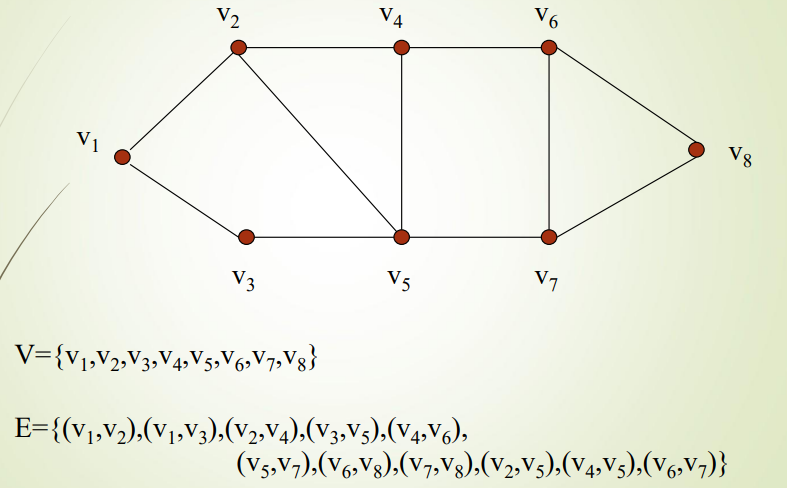
\includegraphics[width = 0.6\textwidth]{figs/grafo.png}
\caption{Ejemplo de grafo de orden 8 y tamaño 11.}
\end{figure}

Para una red de proteínas, cada proteína sería un nodo del grafo, y una rama indicaría interacción entre ambas proteínas. 

Una disposición (layout) es una posible colocación de los nodos y las ramas en un espacio 2D o 3D. Un mismo gráfo puede tener múltiples colocaciones. Ejemplo, consideremos el grafo G=(V,E).

\begin{figure}[h]
\centering
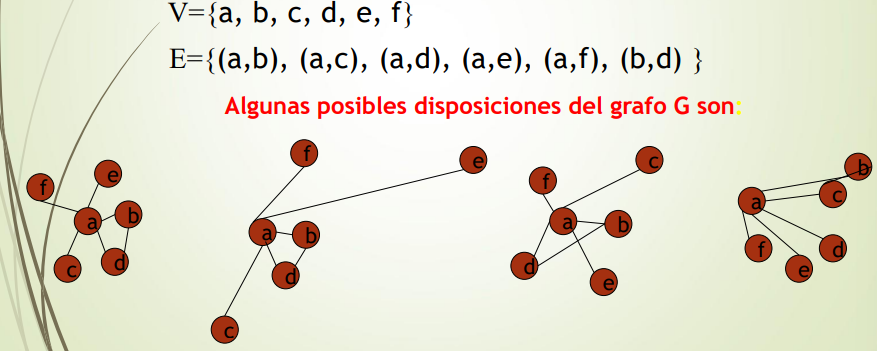
\includegraphics[width = 0.6\textwidth]{figs/layout.png}
\end{figure}

Existen programas de ordenador que nos permiten obtener colocaciones predefinidas (Gephy, Pajek). Cuando no se especifica ninguna colocación, se entiende que los nodos se sitúan aleatoriamente sobre el plano o espacio. Algunos de los tipos más habituales de colocaciones son:
\begin{itemize}
\item Colocaciones regulares
\item Basadas en la física (atracción-repulsión)
\item Basadas en propiedades topológicas (jerarquías, número de vecinos, etc)
\end{itemize}

Un hipergrafo H es un también par de conjuntos (V,E) donde $V=\{v_1, v_2, \ldots v_n\}$ es el conjunto de vértices o nodos y $E=\{(v_{i1}, v_{i2}, \ldots),(v_{i'1},v_{i'2}, \ldots), \ldots\}$ es una familia de
subconjuntos no ordenados de elementos de V. E se denomina conjunto de hiperramas o hiperaristas del hipergrafo. El número de hiperramas $|E|$ se denomina cardinalidad del hipergrafo. El valor $|E|*|V|$ se denomina tamaño o volumen del grafo.
\marginpar[\footnotesize Pregunta examen ]  \
Si tenemos un grafo de n nodos, ¿cuántas parejas podemos tener como máximo? $(n \cdot n-1)/2$ Por tanto, en un grafo con n nodos, ¿cuántas ramas puede tener? Igual, $(n \cdot n-1)/2$

\begin{figure}[h]
\centering
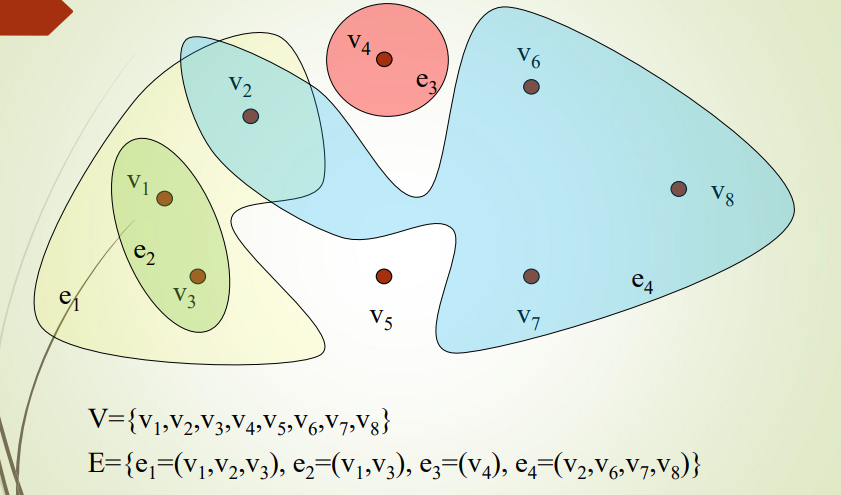
\includegraphics[width = 0.6\textwidth]{figs/hipergrafo.png}
\caption{Ejemplo de hipergrafo de cardinalidad 4 y tamaño 32.}
\end{figure}

Un hipergrafo H se dice que es \textbf{propio} si no es vacío ($V\neq \varnothing$) y no contiene ninguna arista vacía. Un hipergrafo H se dice que tiene \textbf{dominio completo} si todos los nodos están en al menos una arista, en caso contrario se dice que tiene \textbf{dominio parcial}. Si en un hipergrafo todas las hiperramas tienen el mismo número de nodos, entonces se denomina \textbf{hipergrafo k-uniforme}. 

\textit{Ejercicio: Indicar si el hipergrafo del ejemplo anterior es propio, tiene dominio completo y si es k uniforme}. Es propio (el conjunto de vértices tiene 8 elementos y todas las ramas e tienen vértices dentro), es de dominio parcial (v5 no está en ninguna rama) y no es k-uniforme (e1 tiene 3 elementos, e2 tiene 2, e3 tiene 1 y e4 tiene 4).

\section{Bucles y ramas paralelas}
Un bucle es una rama que empieza y termina en el mismo nodo $(v_i, v_i)$. Cuando dos ramas conectan el mismo par de vértices se denominan paralelas. Un grafo con bucles se denomina pseudografo. Un grafo con ramas paralelas pero sin bucles se denomina multigrafos. Un grafo sin bucles ni ramas paralelas se denomina grafo simple.

\begin{figure}[h]
\centering
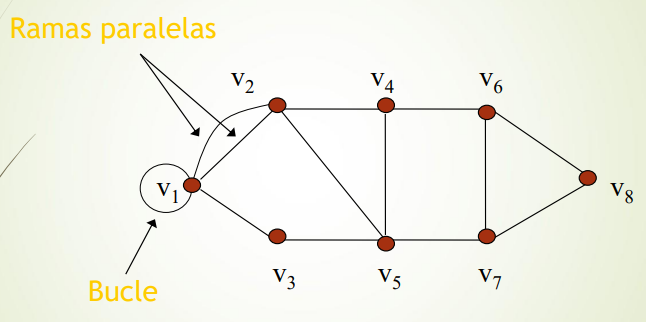
\includegraphics[width = 0.6\textwidth]{figs/bucle-rama-paralela.png}
\end{figure}

%25/03 - Carlos Aguirre
\section{Grafos dirigidos y ponderados}
Se puede considerar que los enlaces entre nodos son dirigidos $(v_i, v_j) = (v_j, v_i)$. Los grafos dirigidos se denominan también \textbf{digrafos}.

\begin{figure}[h]
\centering
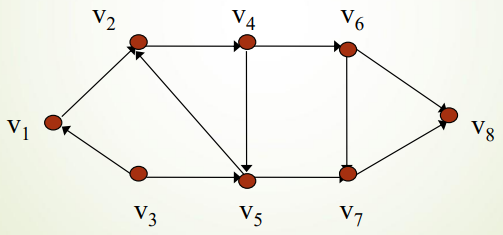
\includegraphics[width = 0.6\textwidth]{figs/grafo-dirigido.png}
\end{figure}

En los grafos ponderados, a cada rama del grafo se le puede asociar un número. El número asociado a cada rama puede indicar entre otras cosas una distancia, una capacidad, un valor temporal, etc.

\begin{figure}[h]
\centering
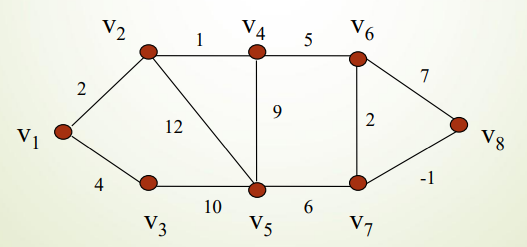
\includegraphics[width = 0.6\textwidth]{figs/grafo-ponderado.png}
\end{figure}

\newpage

Los grafos dirigidos y ponderados poseen ramas dirigidas a las que se asocia un número.

\begin{figure}[h]
\centering
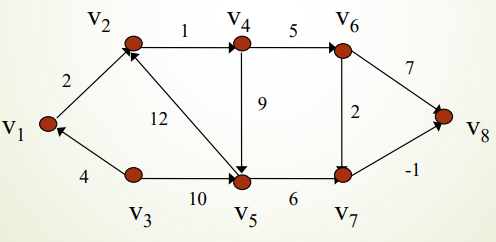
\includegraphics[width = 0.6\textwidth]{figs/grafo-dirigido-ponderado.png}
\end{figure}

\section{Grado de un nodo}
Dos nodos de un grafo son \textbf{vecinos o adyacentes} si existe una rama que los conecta. El \textbf{grado} de un nodo es el número vecinos que tiene dicho nodo. En los grafos dirigidos se calcula el \textbf{grado de entrada} y el \textbf{grado de salida}. En los grafos ponderados, el grado se puede promediar por el número asociado a las ramas. Un grafo se dice que es \textbf{regular} si todos los nodos tienen el mismo grado.

\begin{figure}[h]
\centering
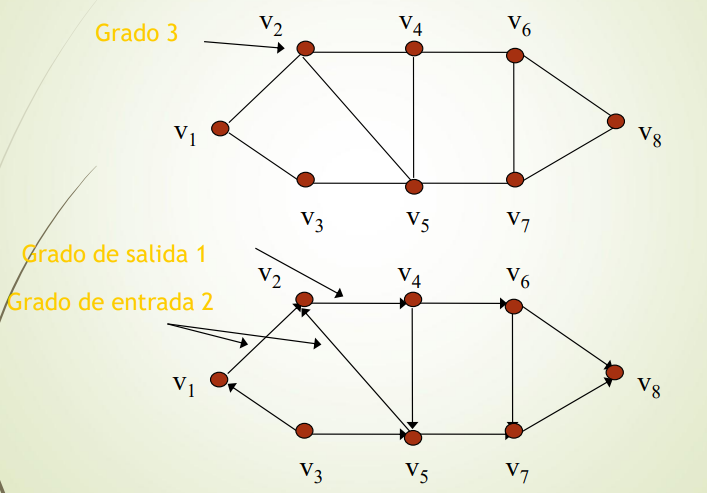
\includegraphics[width = 0.6\textwidth]{figs/grafo-grados.png}
\end{figure}

\section{Subgrafos}
Un grafo G’=(V’,E’) es un subgrafo de un grafo G=(V,E) si V’ es un subconjunto de V y E’ es un subconjunto de E. En otras palabras, un subgrafo es un trozo de un grafo más grande. 

\begin{figure}[h]
\centering
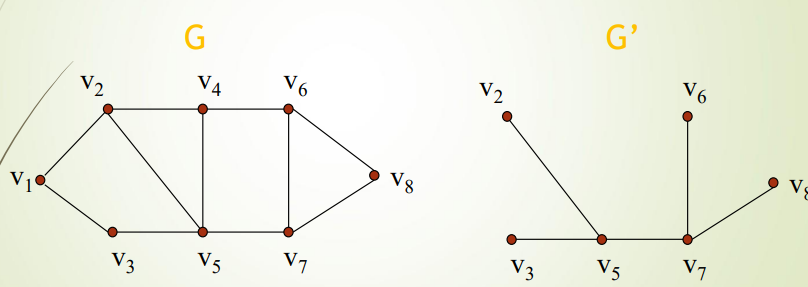
\includegraphics[width = 0.6\textwidth]{figs/subgrafo.png}
\end{figure}

Un subgrafo G’=(V’,E’) de un grafo G=(V,E) se dice que es \textbf{abarcador} si V=V’, es decir, si están todos los nodos, pero faltan algunas ramas.

Un grafo es un subgrafo de sí mismo. Además, un grafo vacío es un subgrafo de cualquier grafo.

\section{Paseos, caminos, circuitos y ciclos}
Un \textbf{paseo} de un nodo u a un nodo v es una secuencia de vértices $\{v_0, v_1, \ldots, v_k\}$ con $v_1 = u v_k = v$ y $(v_{i-1}, v_i)$ rama del grafo. El número de ramas del paseo es su \textbf{longitud}. Un paseo en el cual no se repiten ramas se denomina \textbf{rastro}. Un paseo en el cual todos los vértices $\{v_0, v_1, \ldots, v_k\}$ son distintos se denomina \textbf{camino}. 
Un camino siempre debe ser un rastro y un paseo. Si algo no es rastro, no puede ser camino, y si no es paseo, no puede ser ni rastro ni camino. Cada uno es cada vez más restrictivo.

Entre dos nodos, puede haber varios caminos posibles. Un \textbf{camino mínimo} entre dos nodos es aquel de menor longitud de entre todos los posibles caminos entre ambos nodos. La \textbf{distancia} entre dos nodos del grafo se define como la longitud de cualquier camino mínimo que los una.

\begin{figure}[h]
\centering
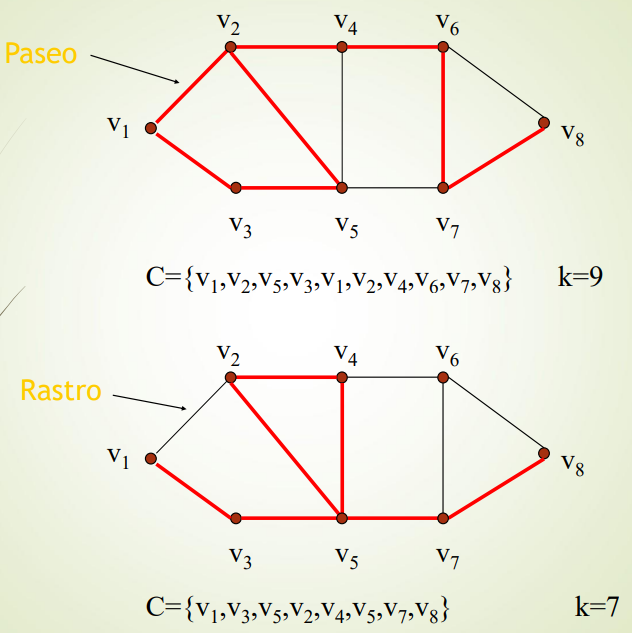
\includegraphics[width = 0.5\textwidth]{figs/paseo-rastro.png}
\end{figure}

\begin{figure}[h]
\centering
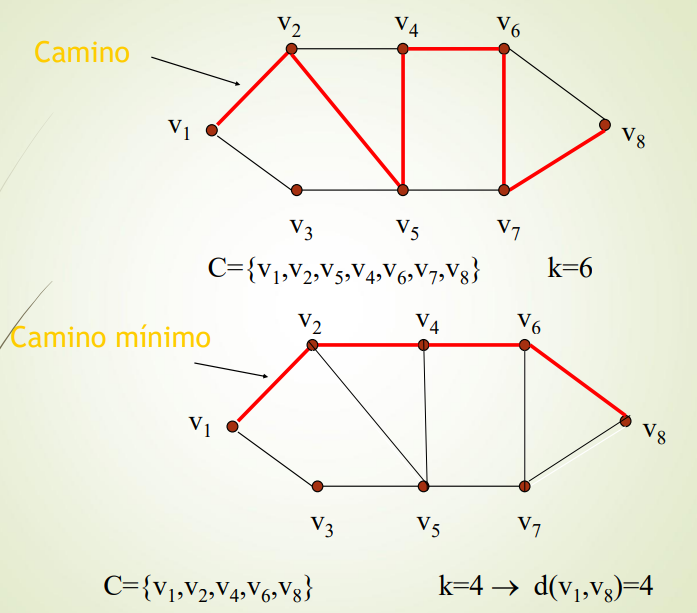
\includegraphics[width = 0.5\textwidth]{figs/camino-minimo.png}
\end{figure}

Un \textbf{paseo cerrado} es un paseo $\{v_0, v_1, \ldots, v_k\}$ tal que $v_0 = v_k$. Un paseo cerrado en el que no se repiten ramas es un \textbf{circuito}. Un \textbf{ciclo} es un circuito en el que no se repiten vértices. Los ciclos son importantes, porque las redes biológicas tienen ciclos (que suelen ser largos), pero en las redes aleatorias no aparecen ciclos, o éstos son muy pequeños.

\begin{figure}[h]
\centering
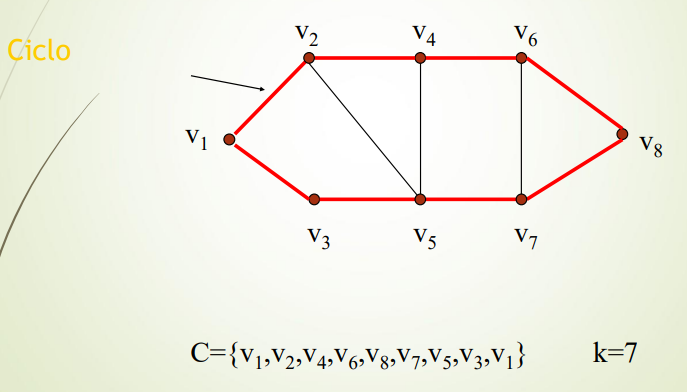
\includegraphics[width = 0.5\textwidth]{figs/ciclo.png}
\end{figure}

El nodo con menor distancia entre los demás es muy importante, denominándose como \textbf{centro del grafo}.

Para un grafo con excesivos nodos, los caminos mínimos y las distancias se calculan con un algoritmo. Si el grafo es no ponderado, se utiliza el algoritmo búsqueda en anchura, mientras que si es ponderado, utiliza Dijkstra.

\section{Medidas de centralidad, betweeness y closeness}
\marginpar[\footnotesize Pregunta examen: Betweeness/Closeness/Farness se define como... ]  \
Dado un nodo $v_i$ se define su \textbf{betweeness} $C_B (v_i)$ como la fracción de caminos mínimos que hay entre el resto de nodos del grafo y que pasan por el nodo $v_i$. Es decir, se hacen parejas de todos los nodos del grafo excluyendo el nodo de interés, y se calculan los caminos mínimos. Algunos pasarán por el nodo de interés, que son los que nos quedamos. Con eso se evalúa el cociente (los que pasan por ese nodo entre todos), que será el betweeness (un valor entre 0 y 1).
La centralidad de un nodo es muy costosa de calcular, usualmente se emplean algoritmos aproximados. 

Dado un nodo $v_i$ se define su \textbf{lejanía o farness} $C_F (v_i)$ como la suma de las distancias de $v_i$ al resto de nodos del grafo. 

Dado un nodo $v_i$ se define su \textbf{cercanía o closeness} $C_C (v_i)$ como la inversa de su lejanía $C_C (v_i) = 1/C_F (v_i)$.

\begin{figure}[h]
\centering
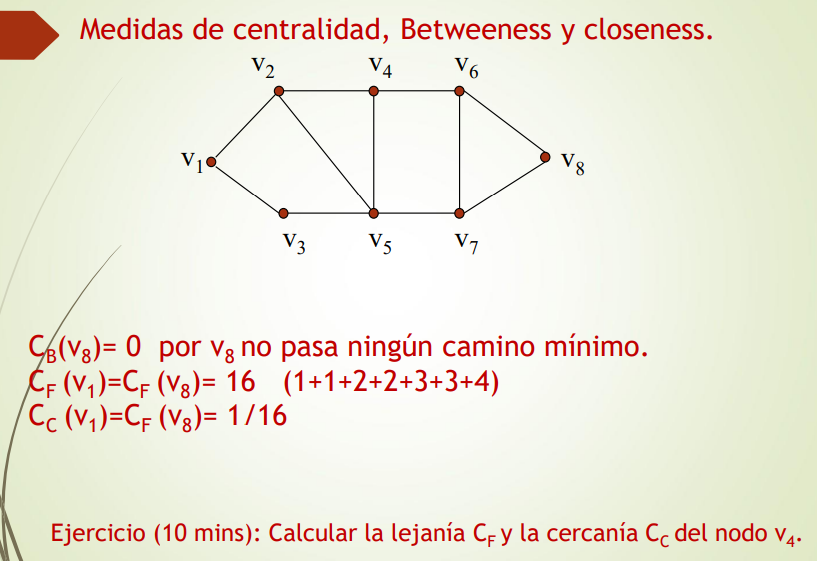
\includegraphics[width = 0.5\textwidth]{figs/medidas-centralidad.png}
\caption{Respuesta al ejercicio: Cogiendo v4, la lejanía será 2+1+2+1+1+2+2 = 11, y la cercanía 1/11.}
\end{figure}

La cercanía y lejanía tiene un problema: su valor numérico depende del orden del grafo. Por tanto, sirve para comparar dentro del mismo grafo, pero no entre grafos. 
\marginpar[\footnotesize Pregunta examen: Calcular camino característico ] \
Para eso, habría que normalizar dividiendo por el número total de nodos. A esto se le conoce como \textbf{camino característico}.

\section{Conexidad}
Un grafo es \textbf{conexo} si para cada par de nodos del grafo existe al menos un camino que los une. En otras palabras, que no esté separado en distintos trozos. 

\begin{figure}[h]
\centering
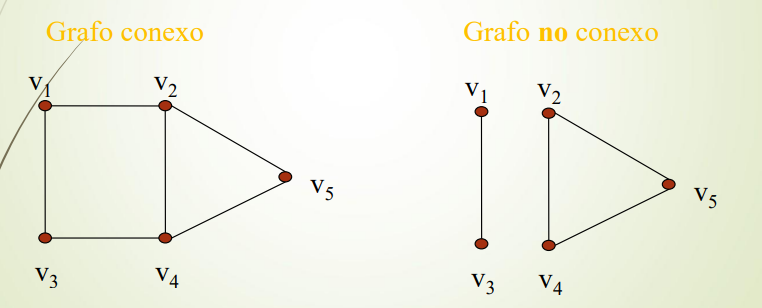
\includegraphics[width = 0.6\textwidth]{figs/conexidad.png}
\end{figure}

Hay un algoritmo muy rápido y eficiente que calcula si un grafo es conexo o no. 

Una \textbf{componente conexa} de un grafo es cada uno de los subgrafos
maximales conexos. Esto quiere decir que el subgrafo no puede ser más grande, que no se le puede añadir más nodos.

\begin{figure}[h]
\centering
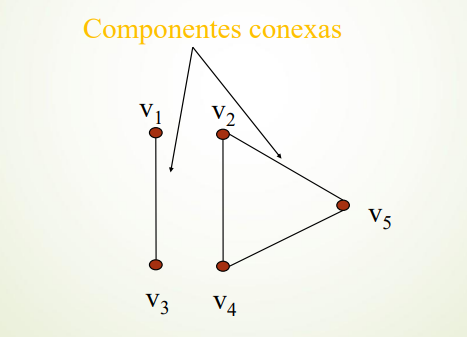
\includegraphics[width = 0.5\textwidth]{figs/componentes-conexas.png}
\end{figure}

Un \textbf{punto de articulación} es un nodo que desconecta un grafo conexo. Un \textbf{corte} es un conjunto de ramas que desconecta un grafo conexo. Si un corte esta compuesto por una única rama, se denomina \textbf{puente}. Un \textbf{corte mínimo} de un grafo es el mínimo número de ramas que al ser eliminadas desconectan el grafo.

El algoritmo CLICK (CLuster Identification via Connectivity Kernels) calcula una aproximación al corte mínimo. Esto lo hacían cogiendo los dos nodos más lejanos. Los puentes suelen ser muy malos para la conexidad de los grafos. 

\begin{figure}[h]
\centering
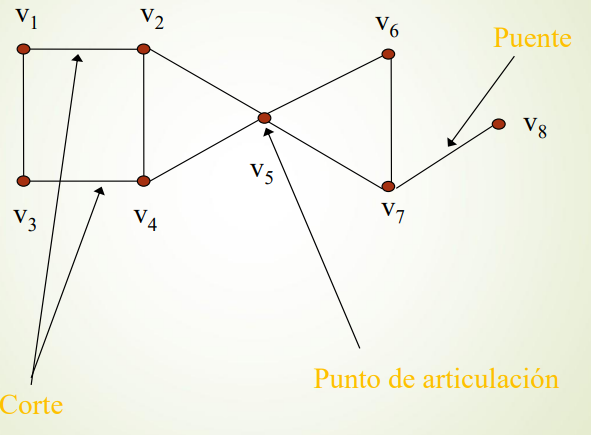
\includegraphics[width = 0.5\textwidth]{figs/conexidad2.png}
\end{figure}

La máxima distancia entre cualquier par de nodos se denomina como diámetro.

El corte mínimo entre dos nodos es siempre mayor que el corte mínimo de todo el grafo.  

\section{Bosques y árboles}
Un grafo sin ciclos (acíclico) se denomina bosque. Un árbol es un grafo acíclico conexo. Cada componente conexa de un bosque es un árbol.

\begin{figure}[h]
\centering
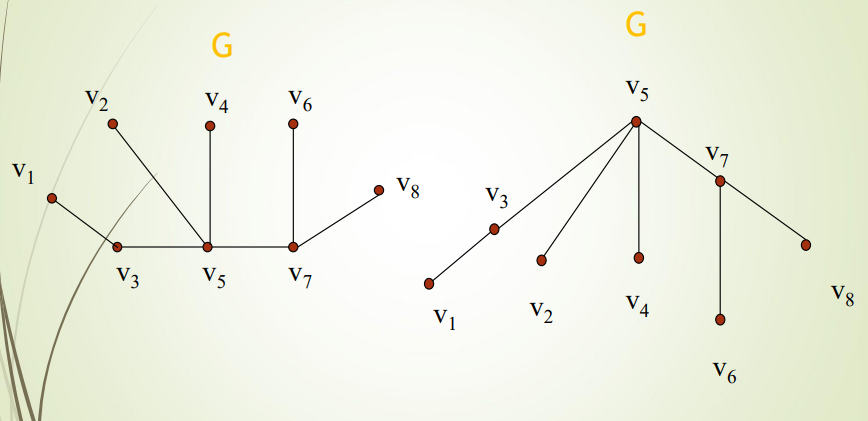
\includegraphics[width = 0.6\textwidth]{figs/arbol-bosque.png}
\end{figure}

Un subgrafo abarcador acíclico de un grafo G se denomina un \textbf{bosque abarcador}. Un subgrafo abarcador conexo acíclico de un grafo G se denomina un \textbf{árbol abarcador}.

\begin{figure}[h]
\centering
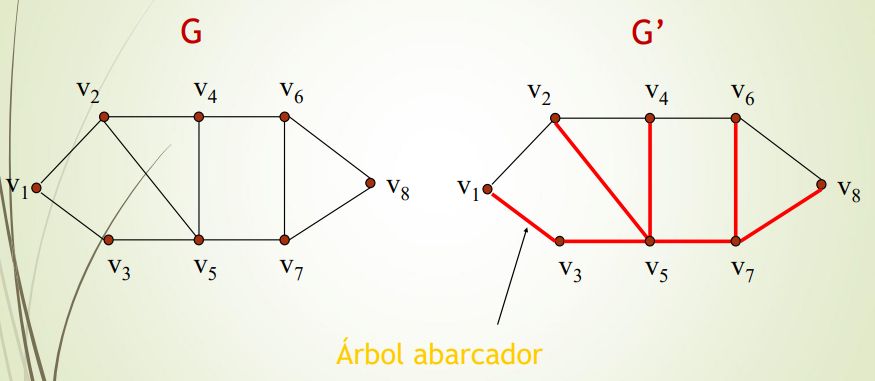
\includegraphics[width = 0.6\textwidth]{figs/arbol-abarcador.png}
\end{figure}


